\section{Triangulations}
Triangulations are a key tool in the process of curve reconstruction.
Specifically, a type of triangulation called a Delaunay triangulation is used to construct the crust of a given set of points.
Before diving into Delaunay triangulations and some interesting results that follow, we first explore an easier problem, the triangulation of a polygon, and build up to Delaunay triangulations from there.

\subsection{Triangulations of Polygons}

To begin, we must first define a triangulation of a polygon.
\begin{definition}[Triangulation of a Polygon] A decomposition of a polygon into triangles by a maximal set of non-intersecting diagonals.
\end{definition}

In simpler terms, a triangulation breaks a polygon into triangular pieces by drawing segments between its vertices so that no two segments intersect.
The term 'maximal set' is used in the definition to ensure that there is no vertex of the polygon on the edge of any triangle.

As an example, let's look at an easy case: a convex octagon.
It is easy to pick out a way to triangulate this shape: just start at one vertex and draw lines to every other vertex as shown in \figref{fig_example_triangulations}.
It is easy to see how this technique can extend to any convex n-gon to create a triangulation with n-2 triangles.
Something of note is that there can be more than one way to triangulate a polygon, with another example shown in \figref{fig_example_triangulations}.
Is it possible that some triangulations are better than others? The fact that there is a section dedicated to a specific type, the Delaunay triangulation, should be a clue here, and the reason why is explored in that section.

\begin{figure}
\[
    \begin{tikzpicture}
      % regular octagon as a node; change minimum size to scale
      \node[
        draw,
        thick,
        regular polygon,
        regular polygon sides=8,
        minimum size=4cm,    % controls overall size
        rotate=22.5          % optional: rotate so a side is horizontal
      ] (oct1) at (-3,0) {};
    
        % regular octagon as a node; change minimum size to scale
      \node[
        draw,
        thick,
        regular polygon,
        regular polygon sides=8,
        minimum size=4cm,    % controls overall size
        rotate=22.5          % optional: rotate so a side is horizontal
      ] (oct2) at (4,0) {};
      
      \foreach \i in {1,...,8}{
        \fill (oct1.corner \i) circle (1.5pt);
        \fill (oct2.corner \i) circle (1.5pt);
      }
      \foreach \i in {1,5,6,7,8}{
        \draw[black, very thick] (oct1.corner 3) -- (oct1.corner \i);
      }
      \draw[black, very thick] (oct2.corner 4) -- (oct2.corner 2);
      \draw[black, very thick] (oct2.corner 4) -- (oct2.corner 1);
      \draw[black, very thick] (oct2.corner 1) -- (oct2.corner 5);
      \draw[black, very thick] (oct2.corner 1) -- (oct2.corner 6);
      \draw[black, very thick] (oct2.corner 8) -- (oct2.corner 6);

    
    \end{tikzpicture}
\]
\caption{Two example triangulations of a regular octagon.} \label{fig_example_triangulations}
\end{figure}

A more interesting problem arises when you try to triangulate a shape that is nonconvex. Is this even possible for \textit{any} polygon? If it is, is there an algorithmic way that works to triangulate any polygon? Will there always be the same number of triangles? The following theorems dive deeper into these questions.

\begin{theorem}All polygons can be triangulated\end{theorem}

\begin{proof}  %This proof comes from computational geometry by springer
	This is an inductive proof with the base case being a polygon with 3 vertices. This base case is trivial because a triangle need not be broken down into more triangular pieces. Now, the assumption that any polygon with $m$ or fewer vertices can be triangulated and our goal is to show that that a polygon with $n$ vertices with $n = m+1 > 3$ can be triangulated.

	I will begin by showing that a diagonal exists in the polygon, $P$, formed by $n$ vertices. Take some vertex $v$ from $P$ and label the vertices neighboring it $u$ and $w$. If $u$ and $w$ are connected and do not intersect with any edges of $P$, then a diagonal exists. Otherwise, there exists one ore more vertices of $P$ that are inside triangle $uvw$. Now, imagine a line parallel to segment $uw$ that goes through $v$. Let this line sweep toward segment $uw$ until it encounters a vertex of $P$ inside triangle $uvw$ and call this vertex $v'$. The segment $vv'$ must be a diagonal because there are no edges of $P$ between $v$ and $v'$ by the definition of $v'$. So, a diagonal must exist in $P$.

	The existence of this diagonal means that $P$ can be broken into two polygons that share the diagonal as a common edge, with a total of $n+2$ vertices. There are $n+2$ because the $n$ outer edges of the polygon remain part of either new polygon, and the diagonal contributes one edge to each of the newly created polygon, adding two edges. Since each new polygon must have at least 3 vertices, the other must have at most $n-1 = m$ vertices. By the inductive hypothesis, each of these new polygons may be triangulated.

	
\newcommand{\nextindex}[3]{%
  % #1 = current index
  % #2 = maximum index
  % #3 = name of variable to store result
  \pgfmathtruncatemacro{\temp}{#1+1}%
  \ifnum\temp>#2
    \pgfmathtruncatemacro{#3}{1}%
  \else
    \pgfmathtruncatemacro{#3}{\temp}%
  \fi
}

\begin{figure}
\[
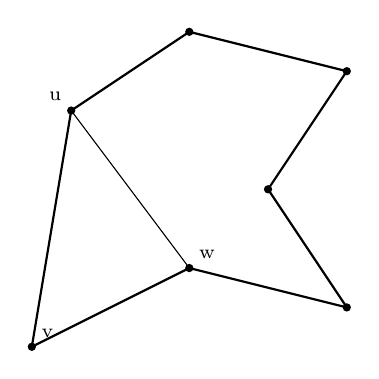
\begin{tikzpicture}[scale=1]
  \coordinate (P1) at (0,0);
  \coordinate (P2) at (2,1);
  \coordinate (P3) at (4,0.5);
  \coordinate (P4) at (3,2);
  \coordinate (P5) at (4,3.5);
  \coordinate (P6) at (2,4);
  \coordinate (P7) at (0.5,3);

  \foreach \i in {1,...,7} {
    \nextindex{\i}{7}{\next}
    \draw[thick] (P\i) -- (P\next);
    \fill (P\i) circle (1.5pt);
  }
  \node[font=\scriptsize, above right] at (P1) {v};
  \node[font=\scriptsize, above right] at (P2) {w};
  \node[font=\scriptsize, above left] at (P7) {u};

  \draw[thin]
    (P2) -- (P7);
  
\end{tikzpicture}
\hspace{3cm}
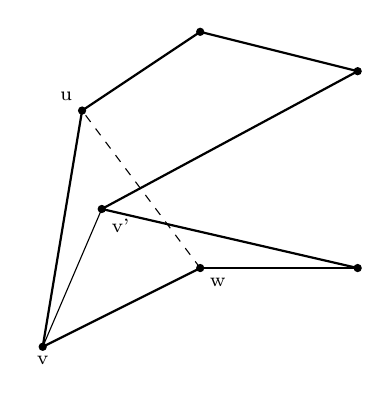
\begin{tikzpicture}[scale=1]
  % --- Define 7 vertices of a nonconvex heptagon ---
  % (Change numbers as you like)
  \coordinate (P1) at (0,0);
  \coordinate (P2) at (2,1);
  \coordinate (P3) at (4,1);
  \coordinate (P4) at (.75,1.75);
  \coordinate (P5) at (4,3.5);
  \coordinate (P6) at (2,4);
  \coordinate (P7) at (0.5,3);

  \foreach \i in {1,...,7} {
    \nextindex{\i}{7}{\next}
    \draw[thick] (P\i) -- (P\next);
    \fill (P\i) circle (1.5pt);
  }
  \node[font=\scriptsize, below] at (P1) {v};
  \node[font=\scriptsize, below right] at (P2) {w};
  \node[font=\scriptsize, above left] at (P7) {u};
  \node[font=\scriptsize, below right] at (P4) {v'};
  
  \draw[dashed]
    (P2) -- (P7);
  \draw[thin]
    (P1) -- (P4);
  
\end{tikzpicture}
\]
\caption{The two cases when trying to draw a diagonal between two points around a starting point.} \label{fig_diagonal_creation}
\end{figure}
\end{proof}

In the process of proving that it is always possible to triangulate any polygon, we have also generated a simple algorithm to triangulate any polygon. If we begin the same way as the proof, drawing a diagonal between some pair of vertices, two smaller shapes are created. Each of these shapes can undergo the same process and create two more shapes. This can be repeated recursively until all the shapes created by the splits are just triangles, so all the diagonals drawn must constitute a triangulation.
\subsection{Triangulations of a Set of Points}

In the previous section, I showed that any polygon can be triangulated. The method to do this started by drawing a single new edge to form a triangle using two preexisting edges. But what if there are no edges at all, and you just have a set of points? You could construct any number of polygons for a given set of points. To make this algorithmic, we must choose a specific one of these polygons to start to triangulate. To do this, we return to the familiar convex hull.

\begin{definition}
	\textbf{Triangulation of a set of Points} FILL OUT THIS DEFINITION
\end{definition}

After computing the convex hull, our situation appears almost like it did in the previous section, but there are still points inside that are not accounted for. To continue down this path, we sincerely hope that the following theorem is true:

\begin{theorem}
	Any set of points $S$ has a triangulation, $T$, such that \textit{Hull(S)}$ \subset T$. --- notation might not be quite right here, we want the edges of the hull to be a part of the edges of T
\end{theorem}

\begin{proof}

	We follow a similar method to the previous proof, using induction. Again, the base case is a set of 3 points, with the obvious triangulation of a triangle, which is also the convex hull of the points. Our hypothesis is that, assuming that a set of points $S$ of size $n$ has triangulation $T$ with \textit{Hull(S)}$ \subset T$, some $S' \supset S$ of size $n+1$ has triangulation $T'$ with \textit{Hull(S')}$ \subset T'$.

	There are two cases for the new vertex $v$ that belongs to $S'$ but not $S$. Either $v$ is inside \textit{Hull(S)}, or it is outside of it. We will examine each case independently:

	Explain that a point outside will have a new hull with two "new edges", and if these two edges are added to the previous triangulation, we still have a triangulation.

	Explain how a point inside the hull is in a triangle, and hence this triangle can just have each vertex connect to the point inside and maintain a triangulation

	...

\end{proof}

\subsection{Delaunay Triangulations}
Now that we know that we can generate some triangulation for any set of points, we can begin to look at a specific type of triangulation, the Delaunay triangulation.
The Delaunay triangulation properties that give it more utility than other triangluations, and is the primary tool in generating the crust.
This section is dedicated to defining it and exploring some interesting results to better understand why it is used to compute the crust.

\begin{definition}[Delaunay Triangluation]
	The triangulation of a set of points $S$ such that the circumcircle of each triangle only contains the vertices of that triangle, and no other points in $S$
\end{definition}
\begin{figure}
\centering

\begin{subfigure}{0.45\textwidth}
\centering
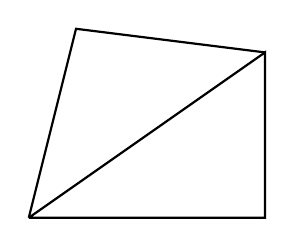
\begin{tikzpicture}[scale=3]
    
    \coordinate (A) at (0,0);
    \coordinate (B) at (1,0);
    \coordinate (C) at (0.2,0.8);
    \coordinate (D) at (1,0.7);
    
    \draw[thick] (A)--(B)--(D)--(A);
    \draw[thick] (A)--(C)--(D);
\end{tikzpicture}
\caption{Non-Delaunay Triangulation}
\end{subfigure}

\hfill

\begin{subfigure}{0.45\textwidth}
\centering
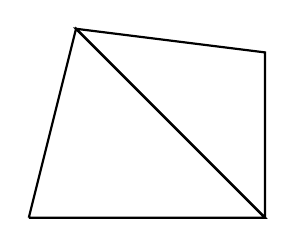
\begin{tikzpicture}[scale=3]    
    % Same points
    \coordinate (A) at (0,0);
    \coordinate (B) at (1,0);
    \coordinate (C) at (0.2,0.8);
    \coordinate (D) at (1,0.7);
    
    % Triangulation (Delaunay: diagonal BC)
    \draw[thick] (A)--(B)--(C)--(A);
    \draw[thick] (B)--(C)--(D)--(B);
\end{tikzpicture}
\caption{Delaunay Triangulation}
\end{subfigure}

\end{figure}


Something you may have noticed in the definition of a Delaunay triangulation is that I claimed that it is \textit{the} triangulation that fits the criteria, not just some triangulation that does.
This uniqueness is an important property of the Delaunay triangulation, but it is not at all apparent.
Unfortunately this feature can be difficult to prove, and must be taken to be true for now.
I will return to this discussion and provide an explanation of this will be provided in the section on Voronoi diagrams.
Taking a step back, we should show that a Delaunay triangulation exists for any set of points, otherwise it would be useless in computational geometry.

Even before proving the existence of the Delaunay triangulation, I must build up to it with a few lemmata.
I will begin by proposing a way to compare triangulations to one another on the basis of the interior angles of their triangles.
Consider two triangulations $T$ and $T'$ of the same set of points $S$, each with $n$ triangles.
Each of these triangulations has a set $A=\{a_1, a_2, ..., a_{3n}\}$ of interior angles, ordered from smallest to largest.
We say that $T>T'$ if $A$ is lexicographically larger than $A'$.

Next, I will introduce three classifications of edges in a triangulation, 'thin', 'fat', and 'locked'.
These classifications come into play when looking at the two triangles adjacent to an edge, making them a local feature of a triangulation, rather than a feature about the whole triangulation itself.
Since these edges have a triangle on each side, they serve as a diagonal of a quadrilateral which I will refer to as the 'surrounding quadrilateral'.
The main idea with these classifications is the relationship with the other diagonal created by the other pair of nonadjacent vertices.
Changing the diagonal of a quadrilateral from one diagonal to the other is considered 'flipping,' which is an idea of great value in the study of triangluations.

\begin{definition}[Thin, Fat, and Locked Edges of a Triangulation]
	A locked edge is an edge whose surrounding quadrilateral is nonconvex, and thus cannot be flipped without violating the definition of a triangulation of a polygon.
	If an edge is not locked, it is a part of some triangulation of $T$ of its surrounding quadrilateral, with $T'$ being the triangulation after flipping.
	An edge is thin if $T<T'$ and fat if $T>T'$
\end{definition}

Now, I will relate the definition of thin and thick edges to the empty circle definition of the Delaunay triangulation.

\begin{lemma}[Thales']
	Consider a circle centered at point $O$ concentric with points $P, Q,$ and $B$.
	For some point $A$ inside the circle and $C$ outside the circle, both on the same side of $P$ and $Q$ as $B$, $\angle PCQ < \angle PBQ < \angle PCQ $.
	(\figref{fig_thales})
\end{lemma}

\begin{figure}
	\[
		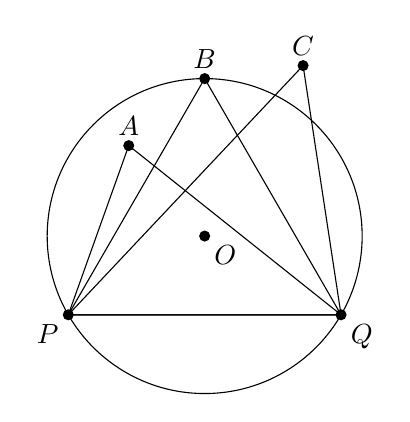
\begin{tikzpicture}[scale=2]
			% Draw the circle
			\draw (0,0) circle (1);

			% Define vertices (TikZ uses degrees)
			\coordinate (O) at (0:0);
			\coordinate (P) at (210:1);
			\coordinate (Q) at (330:1);

			\coordinate (A) at (130:.75);
			\coordinate (B) at (90:1);
			\coordinate (C) at (60:1.25);

			% Draw the triangle
			\draw (P) -- (Q) -- (B) -- cycle;
			\draw (P) -- (Q) -- (A) -- cycle;
			\draw (P) -- (Q) -- (C) -- cycle;

			% Optional: mark the vertices
			\fill (A) circle (1pt);
			\fill (B) circle (1pt);
			\fill (C) circle (1pt);
			\fill (P) circle (1pt);
			\fill (Q) circle (1pt);
			\fill (O) circle (1pt);

			% Labels
			\node[below right] at (O) {$O$};
			\node[below right] at (Q) {$Q$};
			\node[below left] at (P) {$P$};

			\node[above] at (A) {$A$};
			\node[above] at (B) {$B$};
			\node[above] at (C) {$C$};
		\end{tikzpicture}
	\]
	\caption{Three points with the same central angle inside, on, and outside the circle}
	\label{fig_thales}
\end{figure}


\begin{proof}
	It is well known that an inscribed angle is half the central angle. Consider a circle that again goes through $P$ and $Q$, but now goes through $C$.
	This new circle will be centered at a different point, say $O'$.
	This radius of this new circle must be larger than the original since it connects a point outside the original.
	Because $P, Q,$ and $C$ are concentric, $\overline{PO'}=\overline{CO'}=\overline{QO'}$, but $\overline{PQ}$ remains the same as it was in the original circle.
	This means that the isoscles $\triangle PO'Q$ has its equal legs longer than $\triangle POQ$, which implies that the angle between these legs is smaller.
	This smaller angle is the central angle corresponding to the inscribed $\angle PCQ$.
	So since $\angle POQ > \angle PO'Q$, so too is $\angle PBQ > \angle PCQ$.
	The same argument follows for $\angle PAQ > \angle PBQ$.
\end{proof}

\begin{lemma}\label{lem_thin_fat}
	The triangles created by bisecting a quadrilateral are empty of the fourth vertex if and only if the edge bisecting them is thin.
\end{lemma}
\begin{figure}
	\[
		\begin{tikzpicture}[scale=2]
			% Draw the circle
			\draw (0,0) circle (1);

			% Define vertices (TikZ uses degrees)
			\coordinate (A) at (110:1);
			\coordinate (B) at (180:1);
			\coordinate (C) at (275:1);
			\coordinate (D) at (0:.5);

			% Draw the triangle
			\draw (A) -- (B) -- (C) -- (D) -- cycle;
			\draw (A) -- (C);
			\draw (B) -- (D);

			% Optional: mark the vertices
			\fill (A) circle (1pt);
			\fill (B) circle (1pt);
			\fill (C) circle (1pt);
			\fill (D) circle (1pt);

			% angle labels
			\draw pic["$a_1$", draw, angle radius=4mm,angle eccentricity=1.6]
				{angle = A--C--B};
			\draw pic["$b_1$", draw, angle radius=4mm,angle eccentricity=1.6]
				{angle = A--D--B};

			\draw pic["$a_2$", draw, angle radius=4mm,angle eccentricity=1.6]
				{angle = B--A--C};
			\draw pic["$b_2$", draw, angle radius=4mm,angle eccentricity=1.6]
				{angle = B--D--C};

			\draw pic["$a_3$", draw, angle radius=4mm,angle eccentricity=1.6]
				{angle = C--A--D};
			\draw pic["$b_3$", draw, angle radius=4mm,angle eccentricity=1.6]
				{angle = C--B--D};

			\draw pic["$a_4$", draw, angle radius=4mm,angle eccentricity=1.6]
				{angle = D--C--A};
			\draw pic["$b_4$", draw, angle radius=4mm,angle eccentricity=1.6]
				{angle = D--B--A};


			% Labels
			\node[above] at (A) {$A$};
			\node[left] at (B) {$B$};
			\node[below] at (C) {$C$};
			\node[right] at (D) {$D$};
		\end{tikzpicture}
	\]
	\caption{Angle labels used in \lemref{lem_thin_fat}}
	\label{fig_diagonal_labels}
\end{figure}


\begin{proof}
	Consider a convex quadrilateral $ABCD$ with a circle connecting $A, B,$ and $C$, with $D$ inside the circle, and bisect $ABCD$ with its diagonals.
	Label the angles as shown in \figref{fig_diagonal_labels}.
	Since $\triangle ABD$ is inside the circumcircle, $\angle a_1 < \angle b_1$ by Thales' theorem.
	With similar reasoning plus the angle sum of a triangle, $\angle a_2 < \angle b_2, \angle a_3 < \angle b_3,$ and $\angle a_4 < \angle b_4$.
	The 'a' angles correspond to $\overline{AC}$ and the 'b' angles to $\overline{BD}$.
	Since there is some 'b' greater than each 'a', the 'b' angles are lexicographically greater than the 'a' angles, hence $\overline{AC}$ is a thin edge.

	To prove the reverse direction, one can take D is outside the circumcircle and follow the same line of reasoning to show that $\overline{AC}$ must be thick.
\end{proof}

\begin{lemma}
	The Delaunay triangulation contains no thin edges.
\end{lemma}
\begin{proof}
	Since all triangles in a Delaunay triangulation are empty of other points in the set, by the previous corollary, none of the edges may be thin.
\end{proof}

This theorem serves an alternate definition to the Delaunay triangulation.
In some texts, this is the way they are defined, reaching the empty circle property from a series of results in the other direction.
Either way, this result helps expose the property that the Delaunay triangulation is the triangulation that best reduces triangles which are very long and thin.
Perhaps this property serves to make the Delaunay triangulation the 'natural' choice for many applications, ensuring that triangles connect to their "nearest" neighbors, rather than extending far across the shape.

With this new definition, we one step away from proving that the Delaunay triangulation must always exist.
The idea behind this proof is that thin edges can be flipped to thick edges one by one until there are no more thin edges, which makes it a Delaunay triangulation by our new definition.

\begin{theorem}
	A Delaunay triangulation exists for any (finite) set of points $S$.
\end{theorem}
\begin{proof}
	Starting from any triangulation $T$, one may flip any thin edge to a thick edge to create $T'$.
	By the definition of thin and fat edges, a flip will cause the smallest angle in the triangles adjacent to the edge to strictly increase, while leaving all other angles the same.
	As a result, if we call the index of this original smallest angle $i$ in the ordering of the angles in $T$, all angles before $i$ in $T'$ will remain the same, and the value at $i$ will be strictly greater than before.
	This means that after flipping any thin edge to a thick edge to go from $T$ to $T'$, $T' > T$.
	Since there are only a finite number of triangulations of $S$ and flipping thin edges to thick creates a strictly increasing sequence of triangulations, there must be some 'maximum' triangulation where this process must terminate.
	At this 'maximum' triangulation, there must be no thin edges, otherwise there would be some greater triangulation, and if there are no thin edges, the triangulation must be Delaunay.
\end{proof}

So, the existence of the Delaunay triangulation is finally guaranteed.
But it is important to note that this proof still does not guarantee that we have \textit{the} Delaunay triangulation, just that we have \textit{one} of them.
In the process of stepping between increasing triangulations, it would be reasonable to imagine flipping the 'wrong' edge, walking down a path to a local maximum different than if edges are flipped.
It turns out that this is not the case, which is a fascinating convenient result when designing an algorithm to compute the Delaunay triangulation, for we can flip edges in any order and still eventually reach the Delaunay triangulation.
If this were not the case, we would need to put much more care into the design of our algorithm.


It is of note that all the results in this section have dealt with points in \textit{general position}.
If there are four points that are concentric, then there cannot be a triangulation that fits the Delaunay criteria.
So in this case, there is in some sense two valid triangulations that fit the Delaunay criteria which are call these degenerate.
I will not deal with these here since in the general case, randomly sampled points have almost no chance of four concentric points.

